\documentclass[parskip=full]{scrartcl}

\usepackage[utf8]{inputenc}
\usepackage[T1]{fontenc}
\usepackage[ngerman]{babel} %ngermen = new german
\usepackage{glossaries}
\usepackage{float}
\makenoidxglossaries


\newglossaryentry{Feed}{name={Feed},description={Eine Seite, auf der ein Nutzer aktuelle Beiträge sehen kann.}}
\newglossaryentry{App}{name={App},description={App ist eine Abkürzung für das englische Wort Application. Dies Bedeutet Anwendung. Eine App ist also eine Anwendung/Programm, welches eine gewisse Funktion ausführt.}}
\newglossaryentry{AdminRechte}{name={Admin Rechte},description={Der Ersteller einer Veranstaltung oder Gruppe hat diese Rechte. Damit sind die Rechte gemeint, Beiträge aus der Gruppe/Veranstaltung zu löschen oder zu bearbeiten, genauso wie die Rechte die Gruppe/Veranstaltung zu bearbeiten oder zu löschen.}}
\newglossaryentry{Button}{name={Button},description={Ein Knopf der gedrückt werden kann. Dies führt zu einer Aktion}}
\newglossaryentry{Abonnenten}{name={Abonnenten},description={Nutzer die einen abonniert haben}}
\newglossaryentry{Abonnements}{name={Abonnements},description={Nutzer die man abonniert hat}}
\newglossaryentry{GoogleKonto}{name={Google Konto},description={Ein angelegtes Konto bei Google}}
\newglossaryentry{Konversation}{name={Konversation},description={}}
\newglossaryentry{Kategorie}{name={Kategorie},description={Gruppen und Veranstaltungen gehören zu ausgewählten Kategorien. Diese helfen beim Suchen und ordnen der Gruppen und Veranstaltungen}}
\newglossaryentry{Unterkategorie}{name={Unterkategorie},description={Ist eine verfeinerte Kategorie}}



\usepackage{csquotes}
\usepackage{graphicx}
\usepackage{enumitem}

\usepackage[margin=2.5cm]{geometry}
\title{KAnnect}
\subtitle{Pflichtenheft}
\subject{Praxis der Softwareentwicklung}
\titlehead{\centering
\includegraphics[width=6cm]{Logo}}
\author{
	Amani Limame
	\and Zeineb Sbouai
	\and Mohamed Bayoudh
	\and Ibrahim Bouriga
	\and Utku Erol
	\and Florian Giner
}
\date{Sommersemester 2018}
\graphicspath{/home/florian/Documents}
\usepackage{cleveref}
\usepackage{hyperref}
\hypersetup{pdftitle= {PSE: Pflichtenheft,
		bookmarks=true,
	}}
	
	
	
	\begin{document}
		%\input{Deckblatt.tex}
		\maketitle
		\newpage
		\tableofcontents
		\newpage
		\setlength{\parindent}{0em}
		\setlength{\parskip}{0.5em}
		
		\section{Zielbestimmung}
		Die Nutzer sollen durch das Produkt in die Lage versetzt werden, leicht Informationen über Veranstaltungen rund um das Studium am
		KIT und um das Leben in Karlsruhe zu erlangen, sowie sich darüber zu unterhalten.
		
		\subsection{Musskriterien}
		
		\begin{itemize}
			\item Verwalten von Veranstaltungen (Siehe \hyperref[sec:FAVeranstaltungen]{4.3})
			\begin{itemize} 
				
				\item Erstellen, Löschen, Ändern, Suchen, Veranstaltungen abonnieren
				\item Hochladen von einem Bild als Hintergrund
				\item Ersteller hat \gls{AdminRechte}
			\end{itemize}
			
			\item Verwalten von Gruppen (Siehe \hyperref[sec:FAGruppe]{4.2})
			\begin{itemize}
				\item Erstellen, löschen, Ändern, Suchen, Speichern, Gruppen abonnieren
				\item Ersteller hat \gls{AdminRechte}
			\end{itemize}
			\item Verwalten von Kontakten (Siehe \hyperref[sec:FAFreunde]{4.1} und \hyperref[sec:FAKonto]{4.5}) 
			\begin{itemize}
				\item Erstellen, löschen, Ändern, Suchen, Speichern, Kontakte abonnieren
				\item Erstellen des Benutzerkontos über Google Play
			\end{itemize}
			\item In-\gls{App} Kommunikation (Siehe \hyperref[sec:FABeiträge]{4.4} und \hyperref[sec:FANachrichten]{4.6}) 
			\begin{itemize}
				\item versenden, erhalten von Nachrichten
				\item Veröffentlichung von Beiträgen von Nutzern
			\end{itemize}
			\item Beiträge im \gls{Feed} darstellen (Siehe \hyperref[sec:FAFeed]{4.7}) 
			\begin{itemize}
				\item von gefolgten Kontakten/Gruppen/Veranstaltungen
				\item anwenden von Filterkriterien
				\item chronologische Reihenfolge nach Veröffentlichungsdatum
			\end{itemize}
			\item Kommentieren von Beiträgen (Siehe \hyperref[sec:FABeiträge]{4.4}) 
			\begin{itemize}
				\item chronologisch Speichern, löschen, Ändern
			\end{itemize}	
		\end{itemize}
		
		\subsection{Wunschkriterien}
		\begin{itemize}[nosep] 
			\item Sofortige Nachrichtenübermittlung (Siehe \hyperref[sec:FA602]{/FA602/} und \hyperref[sec:FA603]{/FA603/})
			\begin{itemize}
				\item erstellen und löschen von \glspl{Konversation} und Gruppenkonversationen
			\end{itemize}
			
			\item Karte von Karlsruhe (Siehe \hyperref[sec:FA307]{/FA307/})
			\begin{itemize}
				\item zeigt alle Veranstaltungen des heutigen Tages und deren Ort
			\end{itemize}
			\item hochladen von Fotos und Videos (Siehe \hyperref[sec:FA409]{/FA409/})
			\begin{itemize}
				\item für Nutzer
			\end{itemize}
			\item \gls{AdminRechte} sollen weitergegeben werden können an andere Nutzer 
			(Siehe \hyperref[sec:FA504]{/FAFA504/})
			\item Markieren von Nutzern auf Beiträgen (Siehe \hyperref[sec:FA410]{/FA410/})
		\end{itemize}
		
		\newpage
		\subsection{Abgrenzungskriterien}
		\begin{itemize}
			\item Das Produkt soll nur auf Mobilfunk Telefone erhältlich sein.
			\item Das Produkt soll nicht für Handelszwecke genutzt werden.
		\end{itemize}
		\newpage
		
		
		\section{Produkteinsatz}
		Das Produkt soll eine Plattform bereitstellen, die das alltägliche Leben und Studieren in Karlsruhe nicht nur erleichtert, sondern auch verbindet. So sollen Nutzer leicht an Informationen über Veranstaltungen der jeweiligen Hochschule gelangen, wie auch an Informationen über Freizeitaktivitäten. Desweiteren bietet das Produkt noch die Möglichkeit sich leicht darüber zu unterhalten und Meinungen mit anderen Nutzern zu teilen.
		
		\subsection{Anwendungsbereiche}
		\begin{itemize}
			\item Akademischer Bereich
			\item Sozialer Bereich
		\end{itemize}
		
		\subsection{Zielgruppen}
		\begin{itemize}
			\item Studenten
			\item Mitarbeiter der Hochschulen in Karlsruhe
			\item Veranstalter
			% noch für private Personen?
		\end{itemize}
		
		\subsection{Betriebsbedingungen}
		Einsatz des Produkts auf Mobiltelefonen mit einer aktiven Internetverbindung.
		\newpage
		
		\section{Produktumgebung}
		
		\subsection{Software}
			Die \gls{App} wird hauptsächlich für Smartphones entworfen, welches auf Android 4.1 oder höher läuft.
		\subsection{Hardware}
		Handy mit normaler Leistungsfähigkeit
		\newpage
		\section{Funktionale Anforderungen}
		\subsection{Freunde} \label{sec:FAFreunde}
		\begin{itemize}[nosep]
			% Freund suchen
			\item[\textbf{FA100}]\textbf{Freund suchen}
			\newline\newline \textbf{Ziel:} Suche nach einem Freund mithilfe seines Namens
			\newline \textbf{Kategorie:} Primär
			\newline \textbf{Vorbedingungen:} Nutzer muss ein Konto besitzen
			\newline \textbf{Nachbedingungen (Erfolg):} 
			\begin{enumerate}[nosep]
				\item Liste von Personen die den eingetippten Namen haben.
			\end{enumerate}
			\textbf{Nachbedingungen (Fehlschlag):} 
			\begin{enumerate}[nosep]
				\item Wenn keine Person diesen Namen besitzt, wird eine leere Seite mit einer Fehlernachricht angezeigt.
			\end{enumerate}  
			\textbf{Akteure:} Nutzer
			\newline \textbf{Auslösendes Ereignis:} Anfrage des Nutzers
			\newline \textbf{Beschreibung:}
			\begin{enumerate}[nosep]
				\item Im Suchfeld den Name und Vorname eintippen
				\item “Suche” klicken
				\item[3.a.] Eine Liste von Personen mit dem eingetippten Namen wird angezeigt (Erfolg)
				\item[3.b.] Sonst wird eine leere Seite mit einer Fehlernachricht angezeigt (Fehlschlag) \\
			\end{enumerate}
			
						\begin{figure}[H]
							\centering
							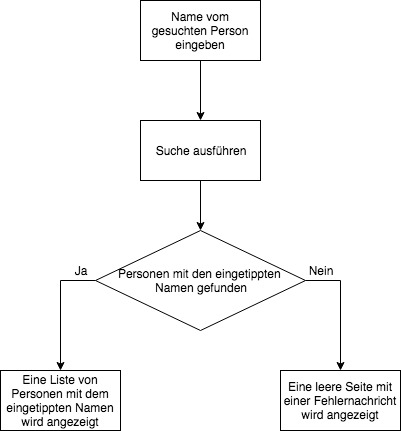
\includegraphics[height=10cm]{Freundsuchen}
							\caption{Zeigt Prozess des Freunde suchens}
							\label{Freundsuchen}
						\end{figure}
			
			\newpage			
			% Freund abonnieren
			\item[\textbf{\large FA101}]\textbf{\large Freund abonnieren}
			\newline\newline \textbf{Ziel:} Beiträge des Freundes angezeigt zu bekommen
			\newline \textbf{Kategorie:} Primär
			\newline \textbf{Vorbedingungen:} Nutzer und Freund müssen ein Konto besitzen
			\newline \textbf{Nachbedingungen (Erfolg):} 
			\begin{enumerate}[nosep]
				\item Freund wird zu der Liste der \gls{Abonnements} des Nutzer hinzugefügt
				\item “Abonnieren” \gls{Button} wird zu “Nicht mehr abonnieren” \gls{Button}
			\end{enumerate}
			\textbf{Nachbedingungen (Fehlschlag):}
			\newline \textbf{Akteure:} Nutzer
			\newline \textbf{Auslösendes Ereignis:} Anfrage des Nutzers
			\newline \textbf{Beschreibung:}
			\begin{enumerate}[nosep]
				\item Zu dem gewünschten Konto Profil navigieren
				\item \gls{Button} “abonnieren” klicken
			\end{enumerate}
			
			% Freund nicht mehr abonnieren
			\item[\textbf{\large FA102}]\textbf{\large Freund nicht mehr abonnieren}
			\newline \textbf{Ziel:} Freund aus der Liste der \gls{Abonnenten} löschen, damit seine Beiträge nicht mehr im \gls{Feed} erscheinen
			\newline \textbf{Kategorie:} Primär
			\newline \textbf{Vorbedingungen:} Freund muss schon abonniert sein
			\newline \textbf{Nachbedingungen (Erfolg):} 
			\begin{enumerate}[nosep]
				\item Freund wird aus der Liste der \gls{Abonnements} des Nutzers gelöscht
				\item “nicht mehr abonnieren” \gls{Button} wird zu “Abonnieren” \gls{Button}
			\end{enumerate}
			\textbf{Nachbedingungen (Fehlschlag):}
			\newline \textbf{Akteure:} Nutzer
			\newline \textbf{Auslösendes Ereignis:} Anfrage des Nutzers
			\newline \textbf{Beschreibung:}
			\begin{enumerate}[nosep]
				\item Zu der Profilseite des Freundes navigieren
				\item Auf \gls{Button} “nicht mehr abonnieren” klicken
			\end{enumerate}
		\end{itemize}
		
			\begin{figure}[H]
				\centering
				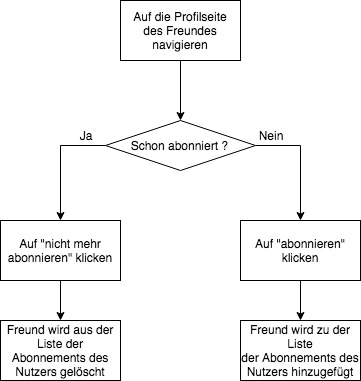
\includegraphics[height=10cm]{Freundediagramm}
				\caption{Zeigt den Prozess des Freunde Abonnierens und nicht mehr Abonnierens}
				\label{Freundediagramm}
			\end{figure}
		
		
		\subsection{Gruppe} \label{sec:FAGruppe}
		\begin{itemize}[nosep]
			%Gruppe erstellen
			\item[\textbf{FA200}]\textbf{Gruppe erstellen}
			\newline \textbf{Ziel:} eine Gruppe erstellen
			\newline \textbf{Kategorie:} Primär
			\newline \textbf{Vorbedingungen:} Nutzer muss angemeldet sein
			\newline \textbf{Nachbedingungen (Erfolg):} 
			\begin{enumerate}[nosep]
				\item Nutzer wird zur Seite der Gruppe weitergeleitet
				\item Gruppe wird zur Liste der gefolgten Gruppen des Erstellers hinzugefügt
				\item Gruppe wird für andere Nutzer sichtbar
			\end{enumerate}
			\textbf{Nachbedingungen (Fehlschlag):}
			\newline \textbf{Akteure:} Nutzer
			\newline \textbf{Auslösendes Ereignis:} Anfrage des Nutzers
			\newline \textbf{Beschreibung:}
			\begin{enumerate}[nosep]
				\item Zur Seite der Gruppen navigieren
				\item Auf \gls{Button} “Gruppe Erstellen” klicken
				\item Ein Formular wird angezeigt , welches ausgefüllt werden muss
				\item Dann auf “Bestätigen” klicken
				\item Nutzer wird nun zur Seite der erstellten Gruppe weitergeleitet\\
			\end{enumerate}
			
			% Gruppe löschen
			\item[\textbf{FA201}]\textbf{Gruppe löschen}
			\newline \textbf{Ziel:} nicht mehr benötigte Gruppen löschen
			\newline \textbf{Kategorie:} Primär
			\newline \textbf{Vorbedingungen:} Gruppe ist schon vorhanden
			\newline \textbf{Nachbedingungen (Erfolg):} 
			\begin{enumerate}[nosep]
				\item Gruppe wird aus System gelöscht
				\item Bestätigungsnachricht wird angezeigt
			\end{enumerate}
			\textbf{Nachbedingungen (Fehlschlag):}
			\newline \textbf{Akteure:} Ersteller der Gruppe
			\newline \textbf{Auslösendes Ereignis:} Anfrage des Erstellers der Gruppe
			\newline \textbf{Beschreibung:}
			\begin{enumerate}[nosep]
				\item Auf die Seite der zu löschende Gruppe navigieren
				\item Auf den \gls{Button} “Löschen” klicken
				\item Aktion bestätigen\\
			\end{enumerate}
			
			% Gruppe beitreten
			\item[\textbf{FA202}]\textbf{Gruppe beitreten}
			\newline \textbf{Ziel:} Gruppenbeiträge angezeigt bekommen und neue Gruppenbeiträge veröffentlichen
			\newline \textbf{Kategorie:} Primär
			\newline \textbf{Vorbedingungen:} Gruppe ist schon vorhanden
			\newline \textbf{Nachbedingungen (Erfolg):} 
			\begin{enumerate}[nosep]
				\item Nutzer wird zu der \gls{Abonnenten}liste der Gruppe hinzugefügt und es wird eine Bestätigungsnachricht angezeigt
				\item ”Gruppe beitreten” \gls{Button} wird zu “aus Gruppe austreten” 
			\end{enumerate}
			\textbf{Nachbedingungen (Fehlschlag):}
			\newline \textbf{Akteure:} Nutzer
			\newline \textbf{Auslösendes Ereignis:} Anfrage des Nutzers
			\newline \textbf{Beschreibung:}
			\begin{enumerate}[nosep]
				\item Auf die Seite der Gruppe navigieren
				\item Auf den \gls{Button} “Beitreten” klicken
				\item Anzeigen einer Bestätigungsnachricht\\
			\end{enumerate}
			
			% Gruppe verlassen
			\item[\textbf{FA203}]\textbf{Gruppe verlassen}
			\newline \textbf{Ziel:} Gruppenbeiträge nicht mehr angezeigt zu bekommen
			\newline \textbf{Kategorie:} Primär
			\newline \textbf{Vorbedingungen:} Benutzer ist Mitglied der vorhandenen Gruppe
			\newline \textbf{Nachbedingungen (Erfolg):} 
			\begin{enumerate}[nosep]
				\item Nutzer wird von der \gls{Abonnenten}liste der Gruppe entfernt
				\item Eine Bestätigungsnachricht wird angezeigt
				\item ”Gruppe verlassen” \gls{Button} wird zu “Gruppe beitreten” 
			\end{enumerate}
			\textbf{Nachbedingungen (Fehlschlag):}
			\newline \textbf{Akteure:} Mitglied der Gruppe
			\newline \textbf{Auslösendes Ereignis:} Anfrage eines Mitglieds der Gruppe
			\newline \textbf{Beschreibung:}
			\begin{enumerate}[nosep]
				\item Auf die Seite der Gruppe navigieren
				\item Auf den \gls{Button} “Verlassen” klicken
				\item Anzeigen einer Bestätigungsnachricht\\
			\end{enumerate}
			
					\begin{figure}[H]
						\centering
						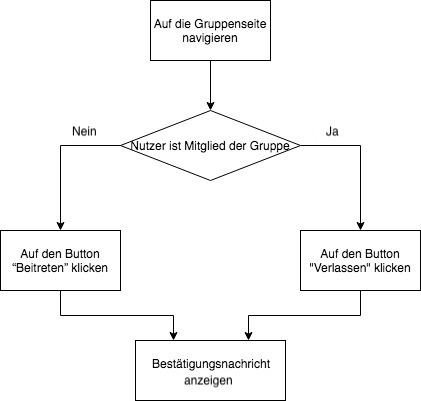
\includegraphics[height=10cm]{Gruppendiagramm}
						\caption{Zeigt den Prozess des Gruppe Bei- und Austretens}
						\label{Freundediagramm}
					\end{figure}	
			
		\end{itemize}
		
		\newpage
		\subsection{Veranstaltungen} \label{sec:FAVeranstaltungen}
		\begin{itemize}[nosep]
			
			%Veranstaltung erstellen
			\item[\textbf{FA300}]\textbf{Veranstaltung erstellen}
			\newline \textbf{Ziel:} Bekanntmachung von Veranstaltungen, Werbemöglichkeit für eine Veranstaltung
			\newline \textbf{Kategorie:} Primär
			\newline \textbf{Vorbedingungen:} Jeder Nutzer kann eine Veranstaltung erstellen
			\newline \textbf{Nachbedingungen (Erfolg):} 
			\begin{enumerate}[nosep]
				\item Veranstaltung wird in die Liste der Veranstaltungen hinzugefügt 
			\end{enumerate}
			\textbf{Nachbedingungen (Fehlschlag):}
			\newline \textbf{Akteure:} Nutzer
			\newline \textbf{Auslösendes Ereignis:} Anfrage des Nutzers
			\newline \textbf{Beschreibung:}
			\begin{enumerate}[nosep]
				\item zu der Seite der Veranstaltungen navigieren
				\item Auf den \gls{Button} “Veranstaltung erstellen” klicken
				\item Formular wird angezeigt, das ausgefüllt werden muss
				\item Auf “Bestätigen” klicken
				\item Nutzer wird zur Seite der Veranstaltung weitergeleitet\\
			\end{enumerate}
			
						\begin{figure}[H]
							\centering
							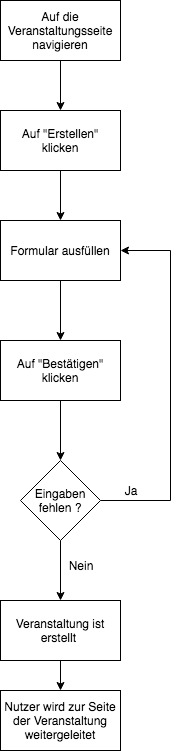
\includegraphics[height=10cm]{Veranstaltungerstellen}
							\caption{Zeigt den Prozess des Veranstaltung Erstellens}
							\label{Veranstaltungerstellen}
						\end{figure}
						
			\newpage
			%Veranstaltung löschen
			\item[\textbf{FA301}]\textbf{Veranstaltung löschen}
			\newline \textbf{Ziel:} Veranstaltung aus dem System löschen
			\newline \textbf{Kategorie:} Primär
			\newline \textbf{Vorbedingungen:} Veranstaltung muss vorhanden sein, Nutzer muss Ersteller sein
			\newline \textbf{Nachbedingungen (Erfolg):} 
			\begin{enumerate}[nosep]
				\item Veranstaltung wird aus Liste der Veranstaltungen gelöscht
				\item Veranstaltung wird aus dem System gelöscht
			\end{enumerate}
			\textbf{Nachbedingungen (Fehlschlag):}
			\newline \textbf{Akteure:}  Nutzer (Ersteller der Veranstaltung)
			\newline \textbf{Auslösendes Ereignis:} Anfrage des Nutzers
			\newline \textbf{Beschreibung:}
			\begin{enumerate}[nosep]
				\item Auf die Seite der Veranstaltung navigieren
				\item Auf den \gls{Button} “Veranstaltung löschen” klicken
				\item Aktion bestätigen
				\item Anzeigen einer Bestätigungsnachricht\\
			\end{enumerate}
			
			%Veranstaltung abonnieren
			\item[\textbf{FA304}]\textbf{Veranstaltung abonnieren}
			\newline \textbf{Ziel:} Neuigkeiten und Informationen der Veranstaltung im \gls{Feed} erhalten
			\newline \textbf{Kategorie:} Primär
			\newline \textbf{Vorbedingungen:} Veranstaltung muss vorhanden sein, Nutzer muss ein Konto haben
			\newline \textbf{Nachbedingungen (Erfolg):} 
			\begin{enumerate}[nosep]
				\item Nutzer wird zu der \gls{Abonnenten}liste der Veranstaltung hinzugefügt
				\item “Veranstaltung abonnieren” \gls{Button} wird zu “ Veranstaltung nicht mehr abonnieren” 
			\end{enumerate}
			\textbf{Nachbedingungen (Fehlschlag):}
			\newline \textbf{Akteure:} Nutzer
			\newline \textbf{Auslösendes Ereignis:} Anfrage des Nutzers
			\newline \textbf{Beschreibung:}
			\begin{enumerate}[nosep]
				\item Auf die Seite der Veranstaltung navigieren
				\item Auf den \gls{Button} “Veranstaltung abonnieren” klicken\\
			\end{enumerate}
			
			
			%Veranstaltung nicht mehr abonnieren
			\item[\textbf{FA305}]\textbf{Veranstaltung nicht mehr abonnieren}
			\newline \textbf{Ziel:} Veranstaltungs Neuigkeiten und Beiträge nicht mehr im \gls{Feed} angezeigt zu bekommen
			\newline \textbf{Kategorie:} Primär
			\newline \textbf{Vorbedingungen:} Nutzer muss die Veranstaltung abonniert haben
			\newline \textbf{Nachbedingungen (Erfolg):} 
			\begin{enumerate}[nosep]
				\item Nutzer wird aus der \gls{Abonnenten}liste der Veranstaltung entfernt
				\item ”Veranstaltung nicht mehr abonnieren” \gls{Button} wird zu “Veranstaltung abonnieren 
			\end{enumerate}
			\textbf{Nachbedingungen (Fehlschlag):}
			\newline \textbf{Akteure:} Nutzer
			\newline \textbf{Auslösendes Ereignis:} Anfrage des Nutzers
			\newline \textbf{Beschreibung:}
			\begin{enumerate}[nosep]
				\item Zur Seite der Veranstaltung navigieren
				\item “Veranstaltung nicht mehr abonnieren” klicken
				\item  Aktion bestätigen\\
			\end{enumerate}
			
			
			\newpage
			%Veranstaltung bearbeiten
			\item[\textbf{FA306}]\textbf{Veranstaltung bearbeiten}
			\newline \textbf{Ziel:} Informationen über die Veranstaltung ändern
			\newline \textbf{Kategorie:} Primär
			\newline \textbf{Vorbedingungen:} Nutzer muss Ersteller der Veranstaltung sein
			\newline \textbf{Nachbedingungen (Erfolg):} 
			\begin{enumerate}[nosep]
				\item Veranstaltung wird geändert 
			\end{enumerate}
			\textbf{Nachbedingungen (Fehlschlag):}
			\newline \textbf{Akteure:} Nutzer
			\newline \textbf{Auslösendes Ereignis:} Anfrage des Nutzers
			\newline \textbf{Beschreibung:}
			\begin{enumerate}[nosep]
				\item Zur Seite der Veranstaltung navigieren
				\item “Veranstaltung bearbeiten” klicken
				\item  Formular wie beim Erstellen wird angezeigt und die Daten können geändert werden
				\item Bearbeitung bestätigen
				\item Nutzer wird zur Seite der Veranstaltung weitergeleitet\\
			\end{enumerate}
			
			
			
			
			
			% Veranstaltung auf Karte ansehen
			\item[\textbf{FA307}]\textbf{Veranstaltung auf Karte ansehen} \label{sec:FA307}	
			\newline \textbf{Ziel:} Herausfinden wo Veranstaltung stattfindet
			\newline \textbf{Kategorie:} Sekundär
			\newline \textbf{Vorbedingungen:} Veranstaltung ist vorhanden und Adresse wurde angegeben
			\newline \textbf{Nachbedingungen (Erfolg):} 
			\begin{enumerate}[nosep]
				\item Veranstaltung wird auf Karte angezeigt
			\end{enumerate}
			\textbf{Nachbedingungen (Fehlschlag):}
			\newline \textbf{Akteure:} Nutzer
			\newline \textbf{Auslösendes Ereignis:} Anfrage des Nutzers
			\newline \textbf{Beschreibung:}
			\begin{enumerate}[nosep]
				\item Auf die Seite der Veranstaltung navigieren
				\item Auf "Auf Karte anzeigen" drücken
				\item Nutzer wird auf die Seite der Karte geleitet\\
			\end{enumerate}
			
			
		\end{itemize}
		
		\subsection{Beiträge} \label{sec:FABeiträge}
		\begin{itemize}[nosep]
			%Beitrag veröffentlichen
			\item[\textbf{FA400}]\textbf{Beitrag veröffentlichen}
			\newline \textbf{Ziel:} Mitteilen von Informationen/Meinungen
			\newline \textbf{Kategorie:} Primär
			\newline \textbf{Vorbedingungen:}
			\newline \textbf{Nachbedingungen (Erfolg):}
			\begin{enumerate}[nosep]
				\item Beitrag wird  veröffentlicht
				\item Beitrag wird auf dem \gls{Feed} der abonnenten des Nutzers angezeigt
			\end{enumerate}
			\textbf{Nachbedingungen (Fehlschlag):}
			\newline \textbf{Akteure:} Nutzer
			\newline \textbf{Auslösendes Ereignis:} Anfrage des Nutzers
			\newline \textbf{Beschreibung:}
			\begin{enumerate}[nosep]
				\item Auf die Hauptseite navigieren
				\item Auf den \gls{Button} “Beitrag erstellen” klicken
				\item Beitrag erstellen
				\item ”Beitrag veröffentlichen” klicken\\
			\end{enumerate}
			
			\newpage
			%Beitrag Gruppe/Veranstaltung veröffentlichen
			\item[\textbf{FA401}]\textbf{Beitrag in Gruppe/Veranstaltung veröffentlichen}
			\newline \textbf{Ziel:} Mitteilen von Informationen/Meinungen in einer Gruppe/Veranstaltung
			\newline \textbf{Kategorie:} Primär
			\newline \textbf{Vorbedingungen:}
			\begin{enumerate}[nosep]
				\item Gruppe/Veranstaltung ist vorhanden,
				\item Gruppe/Veranstaltung ist abonniert vom Nutzer
			\end{enumerate}
			\textbf{Nachbedingungen (Erfolg):}
			\begin{enumerate}[nosep]
				\item Beitrag wird in der Veranstaltung veröffentlicht und auf dem \gls{Feed} der Veranstaltung angezeigt
				\item Beitrag wird auf dem \gls{Feed} der Nutzer angezeigt, die der Veranstaltung folgen
			\end{enumerate}
			\textbf{Nachbedingungen (Fehlschlag):}
			\newline \textbf{Akteure:} Nutzer
			\newline \textbf{Auslösendes Ereignis:} Anfrage des Nutzers
			\newline \textbf{Beschreibung:}
			\begin{enumerate}[nosep]
				\item Auf die Seite der Gruppe/Veranstaltung navigieren
				\item Auf den \gls{Button} “Beitrag erstellen” klicken
				\item Beitrag erstellen
				\item ”Beitrag veröffentlichen” klicken\\
			\end{enumerate}
			
			%Beitrag  löschen
			\item[\textbf{FA402}]\textbf{Beitrag löschen}
			\newline \textbf{Ziel:} Beitrag aus dem System löschen
			\newline \textbf{Kategorie:} Primär
			\newline \textbf{Vorbedingungen:} Nutzer hat den Beitrag verfasst
			\newline \textbf{Nachbedingungen (Erfolg):}
			\begin{enumerate}[nosep]
				\item Beitrag wird aus dem System gelöscht
				\item Beitrag wird nicht mehr angezeigt
			\end{enumerate}
			\textbf{Nachbedingungen (Fehlschlag):}
			\newline \textbf{Akteure:} Ersteller des Beitrags
			\newline \textbf{Auslösendes Ereignis:} Anfrage des Nutzers
			\newline \textbf{Beschreibung:}
			\begin{enumerate}[nosep]
				\item Zu dem zu löschenden Beitrag navigieren
				\item Aktion bestätigen
				\item Anzeigen einer Bestätigungsnachricht
				\item Beitrag verschwindet aus dem \gls{Feed}\\
			\end{enumerate}
			
			%Beitrag in Gruppe/Veranstaltung löschen
			\item[\textbf{FA403}]\textbf{Beitrag in Gruppe/Veranstaltung löschen}
			\newline \textbf{Ziel:} Beitrag aus dem System löschen
			\newline \textbf{Kategorie:} Primär
			\newline \textbf{Vorbedingungen:} Nutzer hat den Beitrag verfasst oder Nutzer ist Ersteller der Gruppe/Veranstaltung
			\newline \textbf{Nachbedingungen (Erfolg):}
			\begin{enumerate}[nosep]
				\item Beitrag wird aus dem System gelöscht
				\item Beitrag wird nicht mehr angezeigt
			\end{enumerate}
			\textbf{Nachbedingungen (Fehlschlag):}
			\newline \textbf{Akteure:} Ersteller der Gruppe/Veranstaltung oder des Beitrags
			\newline \textbf{Auslösendes Ereignis:} Anfrage des Nutzers
			\newline \textbf{Beschreibung:}
			\begin{enumerate}[nosep]
				\item Auf die Seite der Gruppe/Veranstaltung navigieren
				\item Zu dem zu löschenden Beitrag navigieren
				\item Aktion bestätigen
				\item Anzeigen einer Bestätigungsnachricht
				\item Beitrag verschwindet aus dem \gls{Feed} der Veranstaltung\\
			\end{enumerate}
			
			%Beitrag bearbeiten
			\item[\textbf{FA404}]\textbf{Beitrag bearbeiten}
			\newline \textbf{Ziel:} Ein veröffentlichter Beitrag bearbeiten
			\newline \textbf{Kategorie:} Primär
			\newline \textbf{Vorbedingungen:} Beitrag ist vorhanden, Nutzer muss den Beitrag verfasst haben
			\newline \textbf{Nachbedingungen (Erfolg):}
			\begin{enumerate}[nosep]
				\item Beitrag wird geändert
			\end{enumerate}
			\textbf{Nachbedingungen (Fehlschlag):}
			\newline \textbf{Akteure:} Ersteller des Beitrags
			\newline \textbf{Auslösendes Ereignis:} Anfrage des Nutzers
			\newline \textbf{Beschreibung:}
			\begin{enumerate}[nosep]
				\item Zu dem Beitrag navigieren der geändert werden soll
				\item Auf "Beitrag bearbeiten" klicken
				\item Beitrag bearbeiten
				\item "Änderungen speichern" klicken
				\item Beitrag ist geändert\\
			\end{enumerate}
			
			%Beitrag in Gruppe/Veranstaltung bearbeiten
			\item[\textbf{FA405}]\textbf{Beitrag in Gruppe/Veranstaltung bearbeiten}
			\newline \textbf{Ziel:} Ein veröffentlichter Beitrag in einer Gruppe/Veranstaltung bearbeiten
			\newline \textbf{Kategorie:} Primär
			\newline \textbf{Vorbedingungen:} Gruppe/Veranstaltung und Beitrag sind vorhanden, Nutzer muss den Beitrag verfasst haben
			\newline \textbf{Nachbedingungen (Erfolg):}
			\begin{enumerate}[nosep]
				\item Beitrag wird geändert
			\end{enumerate}
			\textbf{Nachbedingungen (Fehlschlag):}
			\newline \textbf{Akteure:} Ersteller des Beitrags
			\newline \textbf{Auslösendes Ereignis:} Anfrage des Nutzers
			\newline \textbf{Beschreibung:}
			\begin{enumerate}[nosep]
				\item Auf die Seite der Gruppe/Veranstaltung navigieren
				\item Zu dem Beitrag navigieren der geändert werden soll
				\item Auf "Beitrag bearbeiten" klicken
				\item Beitrag bearbeiten
				\item "Änderungen speichern" klicken
				\item Beitrag ist geändert\\
			\end{enumerate}
			
			%Beitrag mit "Gefällt mir" markieren
			\item[\textbf{FA406}]\textbf{Beitrag mit "Gefällt mir" markieren}
			\newline \textbf{Ziel:} Zeigen das Beitrag dem Nutzer gefällt
			\newline \textbf{Kategorie:} Primär
			\newline \textbf{Vorbedingungen:} VNutzer muss angemeldet sein, Beitrag muss vorhanden sein
			\newline \textbf{Nachbedingungen (Erfolg):} 
			\begin{enumerate}[nosep]
				\item Anzahl der ‘Gefällt mir’ Angaben des Beitrags wird um eins erhöht
				\item “Gefällt mir” \gls{Button} wird zu “Gefällt mir nicht mehr”
			\end{enumerate}
			\textbf{Nachbedingungen (Fehlschlag):}
			\newline \textbf{Akteure:} Nutzer
			\newline \textbf{Auslösendes Ereignis:} Anfrage des Nutzers
			\newline \textbf{Beschreibung:}
			\begin{enumerate}[nosep]
				\item Zu dem Beitrag navigieren
				\item Auf den \gls{Button} “Gefällt Mir” klicken\\
			\end{enumerate}
			
			
			\newpage
			\item[\textbf{FA407}]\textbf{Beitrag "Gefällt mir nicht mehr"}
			\newline \textbf{Ziel:} Zeigen das Beitrag dem Nutzer nicht mehr gefällt
			\newline \textbf{Kategorie:} Primär
			\newline \textbf{Vorbedingungen:} Beitrag muss vorhanden sein und von dem Nutzer mit "Gefällt mir" markiert sein
			\newline \textbf{Nachbedingungen (Erfolg):} 
			\begin{enumerate}[nosep]
				\item “Gefällt mir nicht mehr” \gls{Button} wird zu “Gefällt mir”
				\item Anzahl der ‘Gefällt mir’ Angaben des Beitrags wird um eins  verringert 
			\end{enumerate}
			\textbf{Nachbedingungen (Fehlschlag):}
			\newline \textbf{Akteure:} Nutzer
			\newline \textbf{Auslösendes Ereignis:} Anfrage des Nutzers
			\newline \textbf{Beschreibung:}
			\begin{enumerate}[nosep]
				\item Zu dem Beitrag navigieren
				\item Auf den \gls{Button} “Gefällt mir nicht mehr” klicken\\
			\end{enumerate}
			
	\begin{figure}[H]
		\centering
		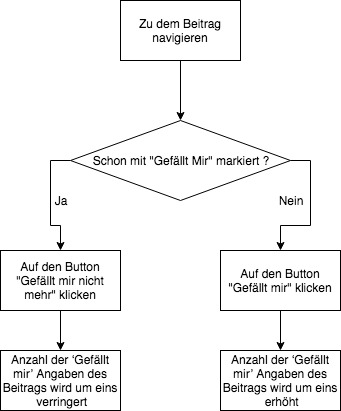
\includegraphics[height=8cm]{beitraggefalltmir}
		\caption{Zeigt den Prozess des Beitrag Gefaellt mir und Gefaellt mir nicht mehr}
		\label{beitraggefalltmir}
	\end{figure}
		
			%Beiträge kommentieren
			\item[\textbf{FA408}]\textbf{Beiträge kommentieren}
			\newline \textbf{Ziel:} Meinungen/Informationen/Reaktion zu einem Beitrag äußern
			\newline \textbf{Kategorie:} Primär
			\newline \textbf{Vorbedingungen:} Nutzer muss eingeloggt sein, Beitrag muss vorhanden sein
			\newline \textbf{Nachbedingungen (Erfolg):} 
			\begin{enumerate}[nosep]
				\item Kommentar wird gespeichert
				\item Kommentar wird unter dem Beitrag angezeigt 
			\end{enumerate}
			\textbf{Nachbedingungen (Fehlschlag):}
			\newline \textbf{Akteure:} Nutzer
			\newline \textbf{Auslösendes Ereignis:} Anfrage des Nutzers
			\newline \textbf{Beschreibung:}
			\begin{enumerate}[nosep]
				\item Zu dem Beitrag navigieren
				\item Auf den ‘Kommentieren’ \gls{Button} klicken
				\item Kommentar schreiben
				\item “Kommentar veröffentlichen” klicken\\
			\end{enumerate}
			
			%Fotos oder Videos als Beitrag veröffentlichen
			\item[\textbf{FA409}]\textbf{Fotos oder Videos als Beitrag veröffentlichen} \label{sec:FA409}
			\newline \textbf{Ziel:} Foto oder Video veröffentlichen
			\newline \textbf{Kategorie:} Sekundär
			\newline \textbf{Vorbedingungen:} Nutzer muss angemeldet sein und die Datei darf nicht größer sein als 10 Megabyte
			\newline \textbf{Nachbedingungen (Erfolg):} 
			\begin{enumerate}[nosep]
				\item Foto/Video werden hochgeladen
				\item Foto/Video wird als Beitrag angezeigt 
			\end{enumerate}
			\textbf{Nachbedingungen (Fehlschlag):} Fehlernachricht wird angezeigt
			\newline \textbf{Akteure:} Nutzer
			\newline \textbf{Auslösendes Ereignis:} Anfrage des Nutzers
			\newline \textbf{Beschreibung:}
			\begin{enumerate}[nosep]
				\item zu dem \gls{Feed} navigieren in dem die Datei hochgeladen werden soll
				\item Auf "Foto/Video veröffentlichen" klicken
				\item Datei auswählen
				\item Aktion bestätigen\\
			\end{enumerate}
			
			%Markieren von Nutzern auf Beiträgen				
			\item[\textbf{FA410}]\textbf{Markieren von Nutzern auf Beiträgen} \label{sec:FA410}
			\newline \textbf{Ziel:} Nutzer auf ein Beitrag aufmerksam machen
			\newline \textbf{Kategorie:} Sekundär
			\newline \textbf{Vorbedingungen:} Die zu markierende Person muss ein Konto besitzen und Beitrag muss vorhanden sein
			\newline \textbf{Nachbedingungen (Erfolg):} 
			\begin{enumerate}[nosep]
				\item Beitrag wird auf dem \gls{Feed} der markierten Person angezeigt 
			\end{enumerate}
			\textbf{Nachbedingungen (Fehlschlag):}
			\newline \textbf{Akteure:} Nutzer
			\newline \textbf{Auslösendes Ereignis:} Anfrage des Nutzers
			\newline \textbf{Beschreibung:}
			\begin{enumerate}[nosep]
				\item Zu dem Beitrag navigieren
				\item Auf den "Kommentieren" \gls{Button} klicken
				\item Im Kommentar @(Name der zu markierenden Person) verwenden
				\item "Kommentar veröffentlichen" klicken\\
			\end{enumerate}
			
		\end{itemize}
		
		\subsection{Konto} \label{sec:FAKonto}
		\begin{itemize}[nosep]
			
			%Konto erstellen
			\item[\textbf{FA500}]\textbf{Konto erstellen}
			\newline \textbf{Ziel:} KAnnect zu benutzen
			\newline \textbf{Kategorie:} Primär
			\newline \textbf{Vorbedingungen:} Nutzer muss ein \gls{GoogleKonto} besitzen und es darf nicht schon ein Konto registriert sein über diesem \gls{GoogleKonto}
			\newline \textbf{Nachbedingungen (Erfolg):} 
			\begin{enumerate}[nosep]
				\item Konto wird erstellt und gespeichert
				\item Nutzer wird zu seinem \gls{Feed} weitergeleitet 
			\end{enumerate}
			\textbf{Nachbedingungen (Fehlschlag):} Eine Fehlernachricht wird angezeigt
			\newline \textbf{Akteure:} Nutzer
			\newline \textbf{Auslösendes Ereignis:} Anfrage des Nutzers
			\newline \textbf{Beschreibung:}
			\begin{enumerate}[nosep]
				\item \gls{App} herunterladen
				\item \gls{App} öffnen
				\item Auf den “Registrieren” \gls{Button} klicken
				\item Mit \gls{GoogleKonto} anmelden und bestätigen\\
			\end{enumerate}
			
			% Konto löschen			
			\item[\textbf{FA501}]\textbf{Konto löschen}
			\newline \textbf{Ziel:} \gls{App} nicht mehr benutzen, alle Daten über Nutzer zu löschen
			\newline \textbf{Kategorie:} Primär
			\newline \textbf{Vorbedingungen:} Nutzer muss ein Konto haben und angemeldet sein
			\newline \textbf{Nachbedingungen (Erfolg):} 
			\begin{enumerate}[nosep]
				\item Nutzerdaten werden von der \gls{App} gelöscht
				\item Nutzer wird abgemeldet 
			\end{enumerate}
			\textbf{Nachbedingungen (Fehlschlag):}
			\newline \textbf{Akteure:} Nutzer
			\newline \textbf{Auslösendes Ereignis:} Anfrage des Nutzers
			\newline \textbf{Beschreibung:}
			\begin{enumerate}[nosep]
				\item Auf das eigene Profil navigieren
				\item Auf “Einstellungen” klicken
				\item Auf “Konto löschen” klicken
				\item Aktion bestätigen\\
			\end{enumerate}
			
			% anmelden				
			\item[\textbf{FA502}]\textbf{anmelden}
			\newline \textbf{Ziel:} \gls{App} benutzen
			\newline \textbf{Kategorie:} Primär
			\newline \textbf{Vorbedingungen:} Nutzer muss registriert sein
			\newline \textbf{Nachbedingungen (Erfolg):} 
			\begin{enumerate}[nosep]
				\item Nutzer wird zu seinem \gls{Feed} weitergeleitet 
			\end{enumerate}
			\textbf{Nachbedingungen (Fehlschlag):}
			\newline \textbf{Akteure:} Nutzer
			\newline \textbf{Auslösendes Ereignis:} Anfrage des Nutzers
			\newline \textbf{Beschreibung:}
			\begin{enumerate}[nosep]
				\item \gls{App} öffnen
				\item Auf den \gls{Button} “Anmelden” klicken
				\item Mit Google-Konto anmelden\\
			\end{enumerate}
			
			% abmelden	
			\item[\textbf{FA503}]\textbf{abmelden}
			\newline \textbf{Ziel:} \gls{App} nicht mehr benutzen oder sich mit einem anderen Kono anmelden
			\newline \textbf{Kategorie:} Primär
			\newline \textbf{Vorbedingungen:} Nutzer ist angemeldet
			\newline \textbf{Nachbedingungen (Erfolg):} 
			\begin{enumerate}[nosep]
				\item Nutzer wird abgemeldet
				\item Nutzer wird zur Anmeldeseite weitergeleitet 
			\end{enumerate}
			\textbf{Nachbedingungen (Fehlschlag):}
			\newline \textbf{Akteure:} Nutzer
			\newline \textbf{Auslösendes Ereignis:} Anfrage des Nutzers
			\newline \textbf{Beschreibung:}
			\begin{enumerate}[nosep]
				\item Zu dem “Abmelden” \gls{Button} navigieren\\
			\end{enumerate}
			
		
			\item[\textbf{FA504}]\textbf{Bearbeitungsrechte weitergeben} \label{sec:FA504}
			\newline \textbf{Ziel:} Bearbeitungsrechte des Erstellers an anderen Nutzer weitergeben
			\newline \textbf{Kategorie:} Sekundär
			\newline \textbf{Vorbedingungen:} Nutzer ist der Ersteller der Gruppe/Veranstaltung
			\newline \textbf{Nachbedingungen (Erfolg):} Der andere Nutzer hat jetzt die Rechte vom Ersteller
			\begin{enumerate}[nosep]
				\item Nutzer wird abgemeldet
				\item Nutzer wird zur Anmeldeseite weitergeleitet 
			\end{enumerate}
			\textbf{Nachbedingungen (Fehlschlag):}
			\newline \textbf{Akteure:} Nutzer
			\newline \textbf{Auslösendes Ereignis:} Anfrage des Nutzers
			\newline \textbf{Beschreibung:}
			\begin{enumerate}[nosep]
				\item Auf der Seite der Gruppe/Veranstaltung navigieren\\
				\item Auf “Verantwortlichen ändern” klicken
				\item Bestätigen
			\end{enumerate}
			
		\end{itemize}
		
		\subsection{Nachrichten} \label{sec:FANachrichten}
		\begin{itemize}[nosep]
			\item[\textbf{FA600}]\textbf{Nachrichten schicken}
			\newline \textbf{Ziel:} Mit anderen Nutzern zu kommunizieren
			\newline \textbf{Kategorie:} Primär
			\newline \textbf{Vorbedingungen:} Nutzer ist angemeldet und Empfänger muss ein Konto haben
			\newline \textbf{Nachbedingungen (Erfolg):} 
			\begin{enumerate}[nosep]
				\item Nachricht wird versendet
				\item Nachricht wird zu dem Ordner “Gesendete Nachrichten” hinzugefügt
			\end{enumerate}
			\textbf{Nachbedingungen (Fehlschlag):}
			\newline \textbf{Akteure:} Nutzer
			\newline \textbf{Auslösendes Ereignis:} Anfrage des Nutzers
			\newline \textbf{Beschreibung:}
			\begin{enumerate}[nosep]
				\item Möglichkeit
				\begin{enumerate}[nosep]
					\item Zum Profil des Empfängers navigieren
					\item “Nachricht schicken” klicken
					\item Nachricht verfassen
					\item Auf den \gls{Button} “Schicken” klicken
				\end{enumerate}
				\item Möglichkeit
				\begin{enumerate}[nosep]
					\item Zum Briefkasten navigieren
					\item “Nachricht schicken” klicken
					\item Empfänger auswählen
					\item Nachricht schreiben
					\item Auf den \gls{Button} “Schicken” klicken\\
				\end{enumerate}
			\end{enumerate}
			
			\item[\textbf{FA601}]\textbf{ Nachrichten empfangen}
			\newline \textbf{Ziel:} Überprüfen ob neue Nachrichten im Briefkasten sind
			\newline \textbf{Kategorie:} Primär
			\newline \textbf{Vorbedingungen:} Nutzer ist angemeldet
			\newline \textbf{Nachbedingungen (Erfolg):} 
			\begin{enumerate}[nosep]
				\item neue Nachrichten werden im Briefkasten angezeigt
				\item Neue Nachrichten können angeklickt und gelesen werden 
			\end{enumerate}
			\textbf{Nachbedingungen (Fehlschlag):}
			\newline \textbf{Akteure:} Nutzer
			\newline \textbf{Auslösendes Ereignis:} Anfrage des Nutzers
			\newline \textbf{Beschreibung:}
			\begin{enumerate}[nosep]
				\item Zum “Briefkasten” navigieren
				\item Auf die neue Nachricht klicken
				\item Nachricht wird geöffnet\\
			\end{enumerate}
			
			
			\newpage
			% Konversation erstellen
			\item[\textbf{FA602}]\textbf{ \gls{Konversation} erstellen} \label{sec:FA602}
			\newline \textbf{Ziel:} Kommunikation mit anderen Nutzern
			\newline \textbf{Kategorie:} Sekundär
			\newline \textbf{Vorbedingungen:} Alle beteiligten Nutzer haben ein registriertes Konto 
			\newline \textbf{Nachbedingungen (Erfolg):} 
			\begin{enumerate}[nosep]
				\item \gls{Konversation} wird erstellt
				\item \gls{Konversation} wird angezeigt 
			\end{enumerate}
			\textbf{Nachbedingungen (Fehlschlag):}
			\newline \textbf{Akteure:} Nutzer
			\newline \textbf{Auslösendes Ereignis:} Anfrage des Nutzers
			\newline \textbf{Beschreibung:}
			\begin{enumerate}[nosep]
				\item Zu "Nachrichten" navigieren
				\item "\gls{Konversation} erstellen" klicken
				\item "Name der \gls{Konversation} eingeben"
				\item Nutzer auswählen die in \gls{Konversation} eingeladen werden sollen
				\item "Bestätigen" klicken
				\item Nutzer wird auf die Seite der \gls{Konversation} geleitet\\
			\end{enumerate}
			
			
			% Konversation löschen
			\item[\textbf{FA603}]\textbf{ \gls{Konversation} löschen} \label{sec:FA603}
			\newline \textbf{Ziel:} Löschen von \gls{Konversation}en
			\newline \textbf{Kategorie:} Sekundär
			\newline \textbf{Vorbedingungen:} \gls{Konversation} muss vorhanden sein, Nutzer muss Ersteller der \gls{Konversation} sein
			\newline \textbf{Nachbedingungen (Erfolg):} 
			\begin{enumerate}[nosep]
				\item \gls{Konversation} wird aus dem System gelöscht
				\item \gls{Konversation} wird nicht mehr angezeigt 
			\end{enumerate}
			\textbf{Nachbedingungen (Fehlschlag):}
			\newline \textbf{Akteure:} Ersteller der \gls{Konversation}
			\newline \textbf{Auslösendes Ereignis:} Anfrage des ERstellers
			\newline \textbf{Beschreibung:}
			\begin{enumerate}[nosep]
				\item Zu "Nachrichten" navigieren
				\item Zu der \gls{Konversation} navigieren
				\item "\gls{Konversation} löschen" klicken
				\item Nutzer wird auf die Seite der Nachrichten geleitet\\
			\end{enumerate}							
		\end{itemize}
		
		\subsection{\gls{Feed}} \label{sec:FAFeed}
		\begin{itemize}[nosep]
			
			% Persönlicher Feed
			\item[\textbf{FA700}]\textbf{persönlicher \gls{Feed}}
			\newline \textbf{Ziel:} Beiträge von abonnierten Veranstaltungen/Freunde und beigetretenen Gruppen zu sehen
			\newline \textbf{Kategorie:} Primär
			\newline \textbf{Vorbedingungen:} Nutzer ist angemeldet
			\newline \textbf{Nachbedingungen (Erfolg):} 
			\begin{enumerate}[nosep]
				\item Beiträge werden im \gls{Feed} angezeigt 
			\end{enumerate}
			\textbf{Nachbedingungen (Fehlschlag):}
			\newline \textbf{Akteure:} Nutzer
			\newline \textbf{Auslösendes Ereignis:} Anfrage des Nutzers
			\newline \textbf{Beschreibung:}
			\begin{enumerate}[nosep]
				\item Zum \gls{Feed} navigieren\\
			\end{enumerate}
		\end{itemize}
		
		
		\newpage
		\section{Produktdaten}
		\begin{itemize}
			\item[\textbf{PD100}] \textbf{Nutzer} \label{sec:PD100}
			\begin{itemize}[nosep]
				\item Name und Vorname
				\item E-Mail
				\item Hochschule
				\item Fachrichtung
				\item Profilbild
				\item \gls{Abonnenten} und \gls{Abonnements} \hyperref[sec:PD100]{(PD100)}
			\end{itemize}
			\item[\textbf{PD200}] \textbf{\gls{Kategorie}} \label{sec:PD200}
			\begin{itemize}[nosep]
				\item Name der \gls{Kategorie}
				\item Gruppen \hyperref[sec:PD300]{(PD300)}
				\item Veranstaltungen \hyperref[sec:PD400]{(PD400)}
				\item \gls{Unterkategorie}n \hyperref[sec:PD201]{(PD201)}
			\end{itemize}
			\item[\textbf{PD201}] \textbf{\gls{Unterkategorie}} \label{sec:PD201}
			\begin{itemize}[nosep]
				\item Name der \gls{Unterkategorie}
				\item Gruppen \hyperref[sec:PD300]{(PD300)}
				\item Veranstaltungen \hyperref[sec:PD400]{(PD400)}
			\end{itemize}
			\item[\textbf{PD300}] \textbf{Gruppe} \label{sec:PD300}
			\begin{itemize}
				\item Name der Gruppe
				\item Beschreibung
				\item Ersteller \hyperref[sec:PD100]{(PD100)}
				\item \gls{Kategorie} \hyperref[sec:P200]{(PD200)} und \gls{Unterkategorie} \hyperref[sec:PD201]{(PD201)}
				\item Profilbild
			\end{itemize}
			\item[\textbf{PD400}] \textbf{Veranstaltung} \label{sec:PD400}
			\begin{itemize}[nosep]
				\item Name der Veranstaltung
				\item Beschreibung
				\item Ersteller \hyperref[sec:PD100]{(PD100)}
				\item \gls{Kategorie} \hyperref[sec:P200]{(PD200)} und \gls{Unterkategorie} \hyperref[sec:PD201]{(PD201)}
			\end{itemize}
			\item[\textbf{PD500}] \textbf{Beitrag} \label{sec:PD500}
			\begin{itemize}[nosep]
				\item Datum
				\item Text
				\item Ersteller \hyperref[sec:PD100]{(PD100)}
				\item Anzahl der "Gefällt mir"
			\end{itemize}
			\item[\textbf{PD600}] \textbf{Nachricht} \label{sec:PD600}
			\begin{itemize}[nosep]
				\item Text
				\item Erstelldatum
				\item Absender \hyperref[sec:PD100]{(PD100)}
				\item Empfänger \hyperref[sec:PD100]{(PD100)}	
			\end{itemize}
		\end{itemize}
		
		\newpage
		\section{Nichfunktionale Anforderungen}
		
		\begin{itemize} 
			\item[\textbf{NFA100}] \textbf{Sicherheit} \label{sec:NFA100}
			\begin{itemize}[nosep]
				\item Kundendaten sollen verschlüsselt werden
			\end{itemize}
			\item[\textbf{NFA200}] \textbf{Zuverlässigkeit} \label{sec:NFA200}
			\begin{itemize}[nosep]
				\item Nicht mehr als ein Ausfall pro Tag
				\item Die \gls{App} soll rund um die Uhr zur Verfüung stehen
			\end{itemize}
			\item[\textbf{NFA300}] \textbf{Erweiterbarkeit} \label{sec:NFA300}
			\begin{itemize}[nosep]
				\item Neue Funktionalitäten sollen sich leicht hinzufügen lassen
			\end{itemize}
			\item[\textbf{NFA400}] \textbf{Benutzbarkeit} \label{sec:NFA400}
			\begin{itemize}[nosep]
				\item Beiträge in chronologischer Reihenfolge anzeigen
				\item Nachrichten in chronologischer Reihenfolge anzeigen
				\item 	Die Menüführung der \gls{App} ist intuitiv für den Nutzer zu bedienen
			\end{itemize}
			\item[\textbf{NFA500}] \textbf{Effizienz und Leistung} \label{sec:NFA500}
			\begin{itemize}[nosep]
				\item Läuft performant auf allen Handys
			\end{itemize}
			\item[\textbf{NFA600}] \textbf{Sprache} \label{sec:NFA600}
			\begin{itemize}[nosep]
				\item Die Texte der GUI sollen in deutscher Sprache verfasst sein
				\item Weitere Sprachen sollen sich leicht hinzufügen lassen
			\end{itemize}
		\end{itemize}	
		
		\newpage
		\section{Globale Testfälle}
		

		\subsection{Allgemein}
		
		\begin{itemize}
			\item[T100] \gls{App} starten
			\begin{enumerate}
				\item
				\begin{enumerate}[nosep]	
					\item Stand: Benutzeroberfläche des Mobiltelefons
					\item Aktion: Aktion Nutzer drückt auf das  Symbol der „KAnnect“ \gls{App}
					\item Reaktion: Reaktion  Seite der Anmeldung wird geöffnet
				\end{enumerate} 
			\end{enumerate}
			
			
			
			\item[T101] Menü öffnen
			Nutzer muss angemeldet sein und darf sich nicht auf der Seite eines Formulars befinden. Auf allen anderen Seiten/Ansichten muss das Menü geöffnet werden können.

		
		
		
		\item[T102] Durch die \gls{App} navigieren
		\begin{enumerate}
			\item
			\begin{enumerate}[nosep]	
				\item Stand: Nutzer muss angemeldet sein und sich nicht auf der Seite des Formulars befinden
				\item Aktion: Nutzer  drückt auf das Menüsymbol
				\item Reaktion:  Das Menü wird geöffnet
			\end{enumerate} 
			\item
			\begin{enumerate}[nosep]	
				\item Stand: Menü ist geöffnet
				\item Aktion: Nutzer drückt auf einen der \gls{Button} im Menü(\gls{Feed}, Profil, Gruppe 1,…)
				\item Reaktion: Nutzer wird zu der dementsprechenden Seite geleitet
			\end{enumerate}
		\end{enumerate}
		
		
		
		\item[T103] Veranstaltungen, Personen und Gruppen suchen
		\begin{enumerate}
			\item
			\begin{enumerate}[nosep]	
				\item Stand: Nutzer muss angemeldet sein und sich auf seinem \gls{Feed} befinden
				\item Aktion: Nutzer  drückt auf das Suchfeld und gibt ein Suchbegriff ein
				\item Reaktion: Es wird eine Liste mit allen Gruppen, Personen und Veranstaltung mit dem angegebenen Suchbegriff angezeigt. Wenn es keine solche Gruppen etc. gibt, wird eine leere Seite mit entsprechender Fehlernachricht angezeigt.
			\end{enumerate} 
		\end{enumerate}
		
		
		
		
		\item[T104]  Hochladen von einem Bild für Veranstaltungen/Gruppen
		\begin{enumerate}
			\item
			\begin{enumerate}[nosep]	
				\item Stand: Formular zum Erstellen einer Veranstaltung oder Gruppe 
				\item Aktion: Nutzer drückt auf „Foto hochladen“
				\item Reaktion:  Es  wird ein Fenster zum Hochladen des Fotos geöffnet
			\end{enumerate} 
			\item
			\begin{enumerate}[nosep]	
				\item Stand: Fenster zum Hochladen des Fotos geöffnet
				\item Aktion: Nutzer sucht das gewünschte Foto und klickt auf „öffnen“
				\item Reaktion: Foto wird hochgeladen und als Profilbild der Veranstaltung/Gruppe gesetzt
			\end{enumerate}
		\end{enumerate}
		
		\item[T105] Anzeigen eines Dialogfensters zum löschen von Veranstaltungen/Gruppen/des Kontos
		\begin{enumerate}
			\item
			\begin{enumerate}[nosep]	
				\item Stand:  Seite der Veranstaltung der Gruppe des eigenen Profils  geöffnet
				\item Aktion: Nutzer drückt auf „Löschen“
				\item Reaktion: Es  wird ein Dialogfenster mit einem \gls{Button} zur Bestätigung des Löschens  angezeigt
			\end{enumerate} 
		\end{enumerate}
		
		\item[T106] Anpassung der Größe von Bildern beim hochladen
		\begin{enumerate}
			\item
			\begin{enumerate}[nosep]	
				\item Stand:  Profil des Nutzers
				\item Aktion: Nutzer  drückt auf „Foto hochladen“, Foto auswählen und bestätigen
				\item Reaktion: Bild in angepasster Größe hochgeladen
			\end{enumerate} 
		\end{enumerate}
		
		\item[T107] Anpassung der Größe der Videos beim Ansehen
		\begin{enumerate}
			\item
			\begin{enumerate}[nosep]	
				\item Stand:  Beitrag mit Video
				\item Aktion: Nutzer  drückt auf das Video
				\item Reaktion: Größe des Videos an das Gerät anpassen(full size)
			\end{enumerate} 
		\end{enumerate}
		
	\end{itemize}
	
	\subsection{Freunde}
	
	\begin{itemize}
		\item[T200] Freund abonnieren
		\begin{enumerate}
			\item
			\begin{enumerate}[nosep]	
				\item Stand: Seite des Nutzers der abonniert werden soll
				\item Aktion: Nutzer klickt auf „Freund abonnieren“
				\item Reaktion: Freund wird zu der Liste der \gls{Abonnements} des Nutzers hinzugefügt. Alle Beiträge des Freundes werden nun im \gls{Feed} des Nutzers angezeigt. \gls{Button} “Freund abonnieren” wird zu “Freund nicht mehr abonnieren”
			\end{enumerate} 
		\end{enumerate}
		
		
		
		\item[T201] Freund nicht mehr abonnieren
		\begin{enumerate}
			\item
			\begin{enumerate}[nosep]	
				\item Stand: Seite des Nutzers der nicht mehr abonniert werden soll
				\item Aktion: Nutzer klickt auf „Freund nicht mehr abonnieren“
				\item Reaktion: Freund wird von der Liste der \gls{Abonnements} des Nutzers gelöscht. Beiträge des Freundes werden nicht mehr auf dem \gls{Feed} des Nutzers angezeigt. \gls{Button} “Freund nicht mehr abonnieren” wird zu “Freund abonnieren”
			\end{enumerate} 
		\end{enumerate}
	\end{itemize}
	
	
	\subsection{Gruppe}
	
	\begin{itemize}
		\item[T300] Erstellen einer Gruppe
		\begin{enumerate}
			\item
			
			\begin{enumerate}[nosep]
				\item Stand: Ansicht Gruppe ist geöffnet
				\item Aktion: Auf “Gruppe erstellen” klicken
				\item Reaktion: Ein Formular zum Erstellen der  Gruppe erscheint
			\end{enumerate}
			\item
			\begin{enumerate}[nosep]	
				\item Stand: Formular zum erstellen einer Gruppe ist geöffnet
				\item Aktion: Daten eingeben und “Bestätigen” klicken
				\item Reaktion: Gruppe wird erstellt und zu den Gruppen hinzugefügt. Nutzer wird zur Seite der Gruppe geleitet
			\end{enumerate}	
		\end{enumerate}
		
		\item[T301] Bearbeiten einer Gruppe
		\begin{enumerate}
			\item
			
			\begin{enumerate}[nosep]
				\item Stand: Seite der Gruppe
				\item Aktion: Ersteller der Gruppe klickt auf “Gruppe bearbeiten”
				\item Reaktion: Das Formular mit allen Informationen über die Gruppe erscheint
			\end{enumerate}
			\item
			\begin{enumerate}[nosep]	
				\item Stand: Formular zum erstellen einer Gruppe ist geöffnet
				\item Aktion:  die Daten ändern (ZB : Name ändern) und “Bestätigen” klicken
				\item Reaktion: Daten werden geändert und Nutzer wird zur Seite der Gruppe geleitet
			\end{enumerate}	
		\end{enumerate}
		
		\item[T302] Gruppe beitreten
		\begin{enumerate}
			\item
			
			\begin{enumerate}[nosep]
				\item Stand: Seite der Gruppe
				\item Aktion:  Auf “Gruppe beitreten” klicken
				\item Reaktion:  Nutzer wird zur Liste der \gls{Abonnenten} der Gruppe hinzugefügt und bekommt alle zukünftigen Beiträge der Gruppe auf seinem \gls{Feed} angezeigt. \gls{Button} “Gruppe beitreten” wird zu “Aus Gruppe austreten”
			\end{enumerate}
			
		\end{enumerate}
		
		\item[T303] Gruppe verlassen
		\begin{enumerate}
			\item
			
			\begin{enumerate}[nosep]
				\item Stand: Seite der Gruppe
				\item Aktion:  Mitglied der Gruppe klickt auf “Aus Gruppe austreten”
				\item Reaktion:   Nutzer wird von der Liste der \gls{Abonnenten} der Gruppe gelöscht. Er bekommt keine Beiträge der Gruppe mehr auf seinem \gls{Feed} angezeigt. \gls{Button} “Aus Gruppe austreten” wird zu “Gruppe beitreten”
			\end{enumerate}
			
		\end{enumerate}		
		
		\newpage
		\item[T304] Gruppe löschen
		\begin{enumerate}
			\item
			
			\begin{enumerate}[nosep]
				\item Stand: Seite der Gruppe
				\item Aktion: Ersteller der Gruppe klickt auf “Gruppe löschen”
				\item Reaktion: Dialogfenster erscheint “Aktion bestätigen”
			\end{enumerate}
			
			\item
			
			\begin{enumerate}[nosep]
				\item Stand: Im Dialogfenster sind die \gls{Button}s « Ja » oder « Nein »
				\item Aktion: Eine Entscheidung Treffen und einer der beiden \gls{Button}s wählen
				\item Reaktion: Wenn « Ja » dann wird Gruppe gelöscht und Ersteller zu seinem \gls{Feed} geleitet
				Wenn  «  Nein » dann wird Ersteller zu der Seite der Gruppe geleitet.
				
			\end{enumerate}
			
		\end{enumerate}		
		
	\end{itemize}
	
	
	\subsection{Veranstaltungen}
	
	\begin{itemize}
		\item[T400] Erstellen einer Veranstaltung
		\begin{enumerate}
			\item
			
			\begin{enumerate}[nosep]
				\item Stand: Ansicht Veranstaltung ist geöffnet
				\item Aktion: Auf \gls{Button} “Veranstaltung erstellen” klicken
				\item Reaktion: Formular zum Erstellen einer Veranstaltung erscheint
			\end{enumerate}
			\item
			\begin{enumerate}[nosep]	
				\item Stand: Formular zum erstellen der Veranstaltung
				\item Aktion: Formular ausfüllen und auf “Bestätigen” drücke
				\item Reaktion: Veranstaltung wird erstellt und zu den Veranstaltungen hinzugefügt. Nutzer wird zur Seite der erstellten Veranstaltung geleitet
			\end{enumerate}	
		\end{enumerate}
		
		\item[T401] Bearbeiten einer Veranstaltung
		\begin{enumerate}
			\item
			
			\begin{enumerate}[nosep]
				\item Stand: Seite der Veranstaltung
				\item Aktion: Ersteller der Veranstaltung klickt auf  “Veranstaltung bearbeiten”
				\item Reaktion: Das Formular mit allen Informationen der Veranstaltung erscheint
			\end{enumerate}
			\item
			\begin{enumerate}[nosep]	
				\item Stand: Formular zum bearbeiten der Veranstaltung
				\item Aktion: Daten ändern (ZB : Name ändern)
				\item Reaktion: Daten werden geändert und Nutzer wird zur Seite der Veranstaltung geleitet
			\end{enumerate}	
		\end{enumerate}
		
		\item[T402] Löschen einer Veranstaltung
		\begin{enumerate}
			\item
			
			\begin{enumerate}[nosep]
				\item Stand: Seite der Veranstaltung
				\item Aktion: Ersteller der Veranstaltung klickt auf “Veranstaltung löschen”
				\item Reaktion:Ein Dialogfenster erscheint “Aktion bestätigen”
			\end{enumerate}
			\item
			\begin{enumerate}[nosep]	
				\item Stand: Dialogfenster mit “Ja” und “Nein” \gls{Button}
				\item Aktion: Eine Entscheidung Treffen und einer der beiden \gls{Button}s klicken
				\item Reaktion: Wenn « Ja » Veranstaltung und alle dazu gehörenden Beiträge aus System gelöscht.
				Wenn  «  Nein »  Ersteller zurück zur Seite der Veranstaltung leiten.
			\end{enumerate}	
		\end{enumerate}
		
		\item[T403] Veranstaltung abonnieren
		\begin{enumerate}
			\item
			
			\begin{enumerate}[nosep]
				\item Stand: Seite der Veranstaltung
				\item Aktion: Nutzer drückt “Veranstaltung abonnieren”
				\item Reaktion:Nutzer wird zur \gls{Abonnenten}liste der Veranstaltung hinzugefügt und bekommt alle zukünftigen Beiträge auf seinem \gls{Feed} angezeigt. “Veranstaltung abonnieren” \gls{Button} wird zu “Veranstaltung nicht mehr abonnieren.
				
			\end{enumerate}
		\end{enumerate}
		
		\newpage
		\item[T404] Veranstaltung nicht mehr abonnieren
		\begin{enumerate}
			\item
			
			\begin{enumerate}[nosep]
				\item Stand: Seite der Veranstaltung
				\item Aktion: Abonnent der Veranstaltung klickt auf “Veranstaltung nicht mehr abonnieren”
				\item Reaktion: Nutzer wird von der Liste der \gls{Abonnenten} gelöscht. Er bekommt keine zukünftige Beiträge der Veranstaltung auf seinem \gls{Feed} angezeigt. \gls{Button} “Veranstaltung nicht mehr abonnieren” wird zu “Veranstaltung abonnieren”
			\end{enumerate}
		\end{enumerate}
		
		\item[T405] Anzeige des Ortes der Veranstaltungen auf der Karte
		\begin{enumerate}
			\item
			
			\begin{enumerate}[nosep]
				\item Stand: Seite der Veranstaltung
				\item Aktion: Auf die Karte navigieren
				\item Reaktion: Eine Karte erscheint dem Standorte der Veranstaltungen
				
			\end{enumerate}
		\end{enumerate}
		
		\item[T406] Synchronisation der Karte beim Erstellen neuer Veranstaltungen
		\begin{enumerate}
			\item
			
			\begin{enumerate}[nosep]
				\item Stand: Seite der Karte
				\item Aktion: Eine neue Veranstaltung erstellen
				\item Reaktion: Die Karte wird aktualisiert und der Standort der neue Veranstaltung wird  hinzugefügt.
				
			\end{enumerate}
		\end{enumerate}
		
	\end{itemize}
	
	
	
	\subsection{Beiträge}
	\begin{itemize}
		\item[T500] Veröffentlichung eines Beitrags
		\begin{enumerate}
			\item
			\begin{enumerate}[nosep]	
				\item Stand: Seite eines \gls{Feed}s
				\item Aktion: Nutzer drückt auf „Beitrag veröffentlichen“
				\item Reaktion: Beitrag wird auf der Seite veröffentlicht und erscheint im \gls{Feed} aller \gls{Abonnenten}
			\end{enumerate} 
		\end{enumerate}
		
		
		\item[T501] Löschen eines Beitrags
		\begin{enumerate}
			\item
			\begin{enumerate}[nosep]	
				\item Stand: Seite auf welcher der Beitrag ist
				\item Aktion: Ersteller klickt auf “Beitrag löschen”
				\item Reaktion: Dialogfenster öffnet sich mit “Aktion bestätigen”
			\end{enumerate} 
			\item
			\begin{enumerate}[nosep]	
				\item Stand: Dialogfenster mit “Aktion bestätigen”
				\item Aktion: Bestätigen oder Aktion abbrechen
				\item Reaktion: \begin{enumerate} [nosep]
					\item Wenn Aktion bestätigt, dann wird Beitrag gelöscht
					\item Wenn Aktion abgebrochen wird, dann wird Nutzer zur Seite des Beitrags geleitet
				\end{enumerate}
			\end{enumerate} 
		\end{enumerate}
		
		\item[T502] Bearbeiten eines Beitrags
		\begin{enumerate}
			\item
			\begin{enumerate}[nosep]	
				\item Stand: Seite des Beitrags
				\item Aktion: Nutzer klickt auf Beitrag bearbeiten
				\item Reaktion: Nutzer kann nun den Text des Beitrags bearbeiten
			\end{enumerate} 
			\item
			\begin{enumerate}[nosep]	
				\item Stand: Nutzer kann Text des Beitrags bearbeiten
				\item Aktion: Nutzer bearbeitet Beitrag und klickt “Änderungen speichern”
				\item Reaktion: Beitrag wird geändert
			\end{enumerate} 
		\end{enumerate}
		
		\newpage
		\item[T503] Kommentieren eines Beitrags
		\begin{enumerate}
			\item
			\begin{enumerate}[nosep]	
				\item Stand: Seite (oder \gls{Feed}) mit Beitrag
				\item Aktion: Nutzer drückt auf „Kommentieren“
				\item Reaktion: Dialogfenster öffnet sich, in welchem das Kommentar verfasst werden kann
			\end{enumerate} 
			\item
			\begin{enumerate}[nosep]	
				\item Stand: Dialogfenster zum Kommentieren
				\item Aktion: Nutzer schreibt sein Kommentar und klickt “Kommentar veröffentlichen”
				\item Reaktion: Kommentar wird veröffentlicht und ist nun unter dem Beitrag sichtbar
			\end{enumerate} 
		\end{enumerate}
		
		\item[T504]  Einen Beitrag nicht mehr mit gefällt mir markieren
		\begin{enumerate}
			\item
			\begin{enumerate}[nosep]	
				\item Stand: Seite (oder \gls{Feed}) mit Beitrag
				\item Aktion: Nutzer drückt auf „Gefällt mir nicht mehr“
				\item Reaktion: Anzahl der “Gefällt mir” wird um eins verringert. \gls{Button} “Gefällt mir nicht mehr” wird zu “Gefällt mir”
			\end{enumerate} 
		\end{enumerate}
		
		
		\item[T505]  Einen Beitrag mit gefällt mir markieren
		\begin{enumerate}
			\item
			\begin{enumerate}[nosep]	
				\item Stand: Seite (oder \gls{Feed}) mit Beitrag
				\item Aktion: Nutzer drückt auf „Gefällt mir“
				\item Reaktion: Anzahl der “Gefällt mir” erhöht sich um eins. \gls{Button} “Gefällt mir” wird zu “Gefällt mir nicht mehr”
			\end{enumerate} 
		\end{enumerate}
		
		
		\item[T506] Beitrag im \gls{Feed} anzeigen, auf welchem der Nutzer markiert wurde
		\begin{enumerate}
			\item
			\begin{enumerate}[nosep]	
				\item Stand:  Beitrag in einem \gls{Feed}
				\item Aktion: Nutzer markiert im Beitrag einen Nutzer
				\item Reaktion: Beitrag erscheint im \gls{Feed} der markierten Person
			\end{enumerate} 
		\end{enumerate} 
	\end{itemize}
	
	
	\subsection{Konto}
	
	\begin{itemize}
		\item[T600] Registrierung mittels Google-Konto
		\begin{enumerate}
			\item
			\begin{enumerate}[nosep]	
				\item Stand: Seite der Registrierung
				\item Aktion:  Auf “Mit \gls{GoogleKonto} registrieren” klicken
				\item Reaktion: Es  wird zur Registrierung mittels Google Account weitergeleitet. Registrierung wird abgewickelt. Nutzer wird dann zu seinem \gls{Feed} weitergeleitet
			\end{enumerate} 
		\end{enumerate}
		
		
		
		\item[T601] Konto löschen
		\begin{enumerate}
			\item
			\begin{enumerate}[nosep]	
				\item Stand: Seite des eigenen Profils
				\item Aktion: Nutzer  drückt auf „Konto löschen“
				\item Reaktion: Dialogfenster wird angezeigt mit “Aktion bestätigen”
			\end{enumerate} 
			\item
			\begin{enumerate}[nosep]	
				\item Stand: Dialogfenster mit “Aktion bestätigen”
				\item Aktion: Nutzer klickt auf „Bestätigen“
				\item Reaktion: Konto wird gelöscht. Nutzer wird zur Seite der Anmeldung geleitet
			\end{enumerate}
		\end{enumerate}
		
		
		
		\item[T602] Anmeldung
		\begin{enumerate}
			\item
			\begin{enumerate}[nosep]	
				\item Stand: Seite Anmeldung
				\item Aktion: Nutzer tippt seine Anmeldedaten ein und klickt auf “Anmelden”
				\item Reaktion:  Nutzer wird zu seinem \gls{Feed} geleitet
			\end{enumerate} 
			\item
			\begin{enumerate}[nosep]	
				\item Stand: Seite Anmeldung
				\item Aktion: Nutzer tippt falsche Anmeldedaten ein und klickt auf “Anmelden”
				\item Reaktion: Fehlermeldung und Nutzer bleibt auf der Anmelde Seite
			\end{enumerate}
		\end{enumerate}
		
		
		\newpage
		\item[T603] Abmeldung
		\begin{enumerate}
			\item
			\begin{enumerate}[nosep]	
				\item Stand: Seite des eigenen Profils
				\item Aktion: Nutzer klickt auf “Abmelden”
				\item Reaktion:  Nutzer wird zur Seite der Anmeldung geleitet
			\end{enumerate} 
		\end{enumerate}
		
		
	\end{itemize}
	
	
	\subsection{Nachrichten}
	
	\begin{itemize}
		\item[T700] Anzeige neuer Nachrichten im Briefkasten
		\begin{enumerate}
			\item
			\begin{enumerate}[nosep]	
				\item Stand:  Seite des Briefkasten
				\item Aktion: Nutzer öffnet Briefkasten
				\item Reaktion: Briefkasten wird aktualisiert und alle emfpangenen Nachrichten werden angezeigt.
			\end{enumerate} 
		\end{enumerate}
		
	\end{itemize}
	\subsection{\gls{Feed}}
	\begin{itemize}
		\item[T701] Anzeigen eines veröffentlichten Beitrags im \gls{Feed} aller \gls{Abonnenten}
		\begin{enumerate}
			\item
			\begin{enumerate}[nosep]	
				\item Stand: \gls{Feed} eines \gls{Abonnenten}
				\item Aktion: Anderen Nutzer den man abonniert hat veröffentlicht ein Beitrag
				\item Reaktion: Beitrag wird im \gls{Feed} des \gls{Abonnenten} angezeigt
			\end{enumerate} 
		\end{enumerate}
		
		\item[T702]  Chronologische Reihenfolge der Beiträge im \gls{Feed}
		\begin{enumerate}
			\item
			\begin{enumerate}[nosep]	
				\item Stand: \gls{App} geöffnet
				\item Aktion: Nutzer  navigiert zu seinem \gls{Feed} oder aktualisiert die \gls{App}
				\item Reaktion:  Alle Beiträge werden  in ein chronologischer Reihenfolge angezeigt
			\end{enumerate} 
			\item
			\begin{enumerate}[nosep]	
				\item Stand: \gls{Feed} des Nutzers
				\item Aktion: Nutzer  drückt auf „Filter“ und wählt  \gls{Kategorie}n aus
				\item Reaktion: Es  wird nur Beiträge von der(n) ausgewählte(n) Filter(n )angezeigt
			\end{enumerate}
		\end{enumerate}
	\end{itemize}
	
	
	\newpage
	\section{Systemmodelle}
	\subsection{Szenarien}
	\subsubsection{Registrierung}
	Bob möchte sich über die Veranstaltungen an den Hochschulen in Karlsruhe informieren, Beiträge von Gruppen sehen und kommentieren. Deswegen geht er auf Google-Play, um eine passende \gls{App} zu finden. Er findet KAnnect und ist sofort überzeugt. Er klickt auf den "Herunterladen" \gls{Button}. Nach der Installation öffnet Bob die \gls{App} und klickt auf “Neues Konto erstellen”. Bob registriert sich erfolgreich mit seinem Google-Konto. Dann wird er zu seinem \gls{Feed} weitergeleitet.
	
	\subsubsection{Freunde}
	Alex ist ein neuer Student in Karlsruhe.  Während der O-Phase hat er einen Kommilitonen kennengelernt, namens Bob. Um die Kommunikation zu erleichtern, hat Bob Alex empfohlen, die neue \gls{App}  KAnnect zu installieren und ihn zu abonnieren. Zu Hause gibt Alex den Namen Bob im Suchfeld ein. Danach klickt er auf den \gls{Button} ‘Abonnieren’. Dadurch bekommt er jetzt alle Beiträge von Bob auf seinem \gls{Feed} angezeigt. Am Wochenende hat Alex Lust mit Bob feiern zu gehen, deswegen hat er ihm eine Nachricht über KAnnect geschrieben. Nach einigen Minuten öffnet er seine Mailbox und sieht, dass er eine Antwort von Bob erhalten hat. Der bestätigt das Treffen in einer Stunde am Schloss. Nach zwei Stunden warten am Schloss, beschließt Alex, sehr erzürnt, heimzugehen. Daheim angelangt geht Alex auf KAnnect und öffnet Bobs Profil und klickt “nicht mehr abonnieren”.
	
	\subsubsection{Gruppen}
	Die neue Hochschulgruppe „Technologien für Studenten“ möchte ihre Neuigkeiten den Studenten präsentieren. Alex, ein Verantwortlicher der Gruppe meldet sich mit seinem Konto an. Er drückt in der \gls{App} auf “Gruppe erstellen” und muss nun ein Formular ausfüllen. Nachdem er das gemacht hat, drückt er “Bestätigen” und die Gruppe wird zu der Liste der gefolgten Gruppen hinzugefügt %Link zu GUI
	Bob ist ein Student und interessiert sich für diese Gruppe. Er meldet sich in der \gls{App} an und gibt den Namen der Gruppe in das Suchfeld ein. Nun wird ihm die gesuchte Gruppe angezeigt. Er klickt auf „Gruppe beitreten“ und kann nun alle Beiträge in der Gruppe sehen. Diese werden ihm nun auch in seinem \gls{Feed} angezeigt. Bob fragt sich, wie man Mitglied der Hochschulgruppe werden kann, weshalb er einen Beitrag in der Gruppe veröffentlicht. Nach rund fünf Minuten sieht Alex den Beitrag von Bob und erklärt den Bewerbungsprozess, indem er den Beitrag kommentiert. Da Alex davon ausgeht, dass noch mehr Leute dieselbe Frage haben, verfasst er einen Beitrag über den Bewerbungsprozess und veröffentlicht diesen in der Gruppe. Nach der Veröffentlichung bemerkt Alex, dass er einen veralteten Prozess erläutert hat. Deswegen klickt er auf „Beitrag löschen“.
	Da Bob nach einer Woche immer noch keine richtige Antwort erhalten hat, tritt er aus der Gruppe aus.
	Bob bemerkt, dass seine Gruppe “O-Phase 2014” nicht mehr aktiv ist, und will sie löschen. Er geht auf der Seite der Gruppe und klickt auf „Gruppe löschen“. Nachdem er “Bestätigen” klickt, wird die Gruppe gelöscht.
	
	\subsubsection{Veranstaltungen}
	Manfred Maier ist ein Student in Karlsruhe. Die Klausurenphase ist endlich vorbei. Er hat Lust heute Nachmittag etwas zu machen, aber weiß nicht genau was. Er fragt seinen besten Freund Siegfried, was heute in Karlsruhe abgeht. Leider kann er auch nichts Besonderes vorschlagen und sagt, dass sie KAnnect checken sollen. Manfred denkt, dass es eine sehr gute Idee ist, und öffnet die \gls{App}.
	Auf der Hauptseite klickt er auf den \gls{Button} "Veranstaltungen" und befindet sich nun auf einer neuen Seite, auf der alle Veranstaltungen nach Datum sortiert sind. Oben sind die Veranstaltungen, die heute stattfinden werden, weiter unten die der kommenden Tage und Wochen.
	Da ihm so viele Veranstaltungen angezeigt werden, will er die Veranstaltungen filtern. Er klickt auf "eine Veranstaltungskategorie wählen" und sieht alle \gls{Kategorie}n wie "Sport" "Studium" "Nightclubs" "Bars \& Pubs" "Essen" usw. 
	Dann wählt er "Bars \& Pubs" und die Seite aktualisiert sich. Nun werden nur die Veranstaltungen angezeigt, die etwas mit der \gls{Kategorie} zu tun haben.
	Er sieht, dass eine Bar heute von 17 bis 19 Uhr Happy Hour mit Live Musik anbietet. Er klickt auf die Veranstaltung, um weitere Details zu sehen. Er befindet sich nun auf der Seite der Veranstaltung. Dort werden ihm veröffentlichte Beiträge der Veranstaltung angezeigt. Nach einer kurzen Diskussion, entscheiden sich Manfred und Siegfried in diese Bar zu gehen. Um neue Informationen über die Veranstaltung in seinem \gls{Feed} angezeigt zu bekommen, klickt Manfred auf "Veranstaltung abonnieren". Außerdem wollen sie später noch zu irgendeiner Party gehen. Ganz oben auf der Veranstaltungsseite ist ein Suchfeld "Veranstaltungen suchen". Da gibt er "Party" ein und die Seite aktualisiert sich. Nun werden ihm alle Veranstaltungen die das Schlüsselwort "Party" haben angezeigt. Er mag diese Veranstaltungen nicht und entscheidet sich, eine eigene Party zu schmeißen. Er redet mit Siegfried und sie machen die Partyvorbereitungen zusammen. Sie wollen jeden einladen, der mitfeiern will. Er geht auf "Erstelle neue Veranstaltung" und bekommt ein Formular von der \gls{App}: 
	
	%link zu gui
	
	Nachdem er es fertig ausgefüllt hat, bestätigt er das Erstellen der Veranstaltung und wird zu der Seite seiner Veranstaltung weitergeleitet. Er kontrolliert die Seite noch mal und sieht, dass er eine falsche Adresse eingegeben hat. Er klickt auf "Veranstaltung bearbeiten" und wird wieder zu dem Formular geleitet.Nun korrigiert er seinen Fehler und bestätigt seine Änderungen und kommt wieder zurück zu der Veranstaltungsseite.
	
	Eine Woche später möchte er wieder so eine Party schmeißen und erstellt wieder eine neue Veranstaltung in der \gls{App}. Am nächsten Tag bekommt er seine Klausurergebnisse und ihm gefallen seine Noten überhaupt nicht. Deswegen möchte er sich mehr auf sein Studium konzentrieren und sagt die Party ab. Er öffnet KAnnect und navigiert auf die Seite seiner erstellten Veranstaltung. Dann klickt er auf “Veranstaltung löschen”.
	
	\subsubsection{\gls{Feed}}
	Bob öffnet KAnnect und möchte sein \gls{Feed} durchschauen. Er sieht die Beiträge seiner Freunde, seiner abonnierten Veranstaltungen und seiner gefolgten Gruppen in chronologische Reihenfolge.
	Bob will auf ein Beitrag reagieren , er klickt “Gefällt mir”, weil ein Freund von ihm was Lustiges gepostet hat. Er ist die 16.te Person, die den Beitrag mit “Gefällt mir” markiert hat. Außerdem kommentiert er den Beitrag, daraufhin merkt er, dass auch diese chronologisch sortiert sind.
	
	\newpage
	\subsection{Anwendungsfälle}
	
		\begin{figure}[H]
			\centering
			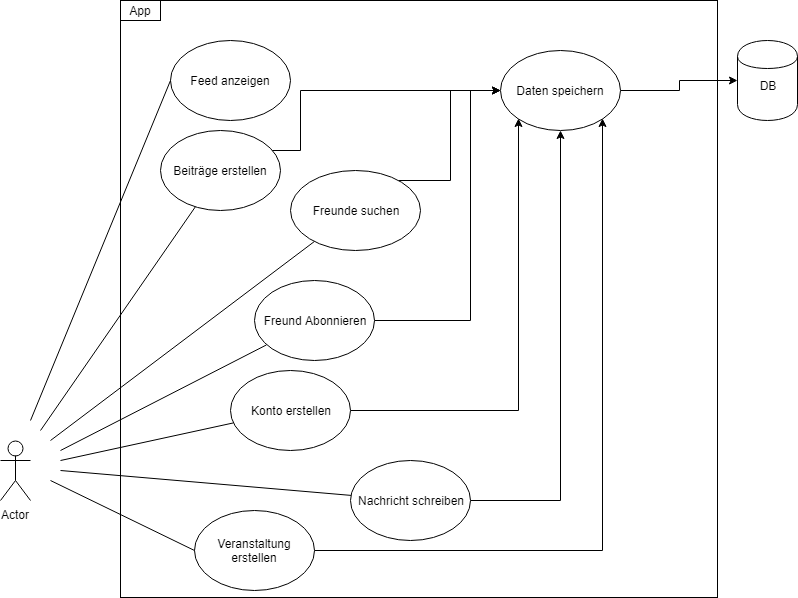
\includegraphics[height=12cm]{Anwendungsfalldiagramm}
			\caption{Zeigt Zusammenhang zwischen Aktionen des Nutzers und der Datenbank}
			\label{Anwendungsfalldiagramm}
		\end{figure}
		
		
	\newpage
	\section{Grafische Benutzeroberfläche}
	Die folgenden Darstellungen der Benutzeroberfläche sind Skizzen und dienen zum Verdeutlichen des groben Aufbaus der \gls{App}. Das Endprodukt kann von ihnen abweichen.
	Die dargestellten Ansichten sind: 
	\begin{itemize}
		\item Abbildung \ref{Registrierung} Registrierung
		\item Abbildung \ref{PersönlicherFeed} \gls{Feed}: Dies ist die Hauptansicht. Der Nutzer wird zu dieser Ansicht weitergeleitet nachdem er sich registriert oder angemeldet hat.
		\item Abbildung \ref{Menü} zeigt das Menü. Mit diesem kann der Nutzer durch die \gls{App} navigieren
		\item Abbildung \ref{OffenesMenü} geöffnetes Menü: Im Hintergrund ist der \gls{Feed} (Abbildung \ref{PersönlicherFeed}) dargestellt
		\item Abbildung \ref{Veranstaltung} Veranstaltung
		\item Abbildung \ref{FormularVeranstaltung} Formular: Muss ausgefüllt werden um eine Veranstaltung zu erstellen. Ein ähnliches Formular wird zum erstellen einer Gruppe angezeigt
		\item Abbildung \ref{Gruppe} Gruppe
		\item Abbildung \ref{BeitragMitKommentaren} zeigt ein Beitrag und die dazugehörende Kommentare
		\item Abbildung \ref{Briefkasten} Briefkasten
		\item Abbildung \ref{Nachricht} Nachricht verfassen
	\end{itemize}
		
	
	\begin{figure}[H]
		\centering
		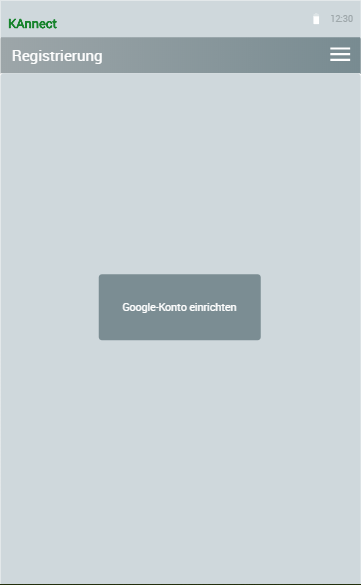
\includegraphics[height=8cm]{Registrierung}
		\caption{Registrierung}
		\label{Registrierung}
	\end{figure}
	
	\begin{figure}[H]
		\centering
		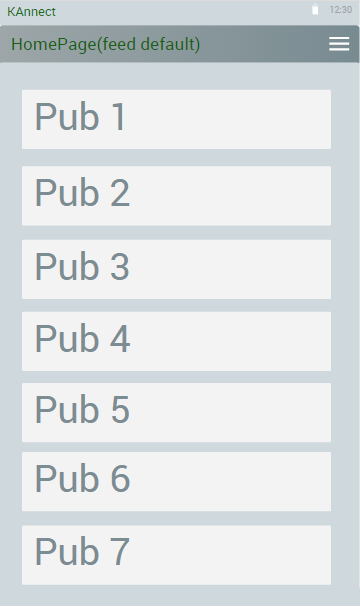
\includegraphics[height=8cm]{PFeed}
		\caption{Persönlicher Feed}
		\label{PersönlicherFeed}
		\hypertarget{PFeed}{}
	\end{figure}
	
	\begin{figure}[H]
		\centering
		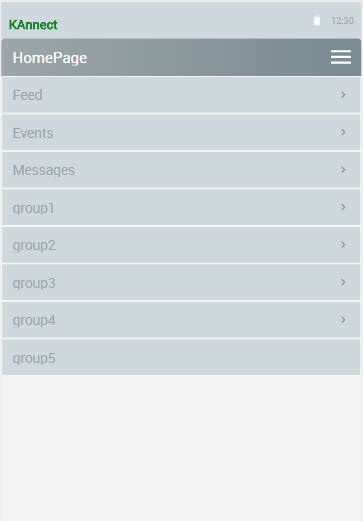
\includegraphics[height=8cm]{Menu}
		\caption{Menü}
		\label{Menü}
	\end{figure}
	
	\begin{figure}[H]
		\centering
		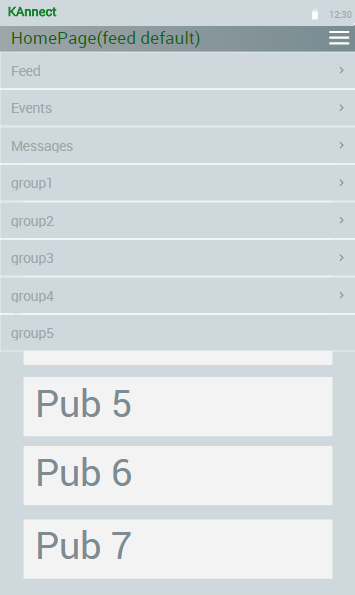
\includegraphics[height=8cm]{MenuOpened}
		\caption{Geöffnetes Menü}
		\label{OffenesMenü}
	\end{figure}
	
	\begin{figure}[H]
		\centering
		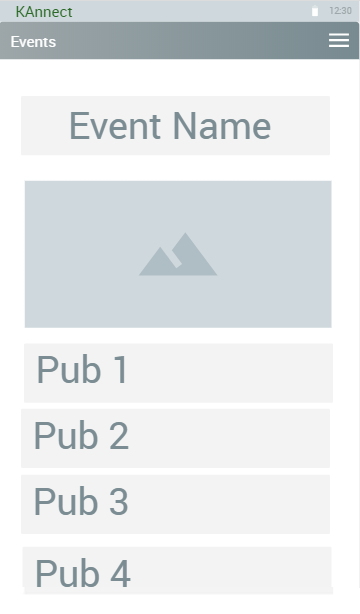
\includegraphics[height=8cm]{Event}
		\caption{Veranstaltung}
		\label{Veranstaltung}
	\end{figure}
	
	
	\begin{figure}[H]
		\centering
		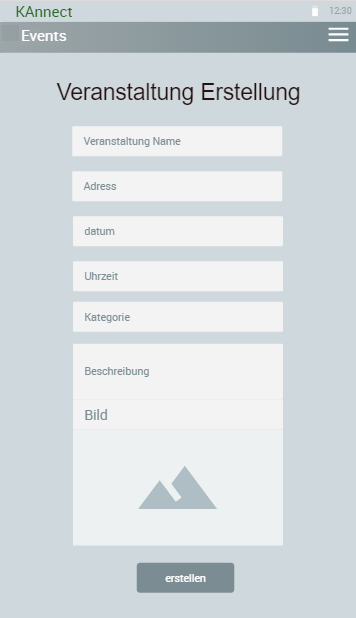
\includegraphics[height=8cm]{FormularVeranstaltung}
		\caption{Formular zum erstellen einer Veranstaltung}
		\label{FormularVeranstaltung}
	\end{figure}
	
	
	\begin{figure}[H]
		\centering
		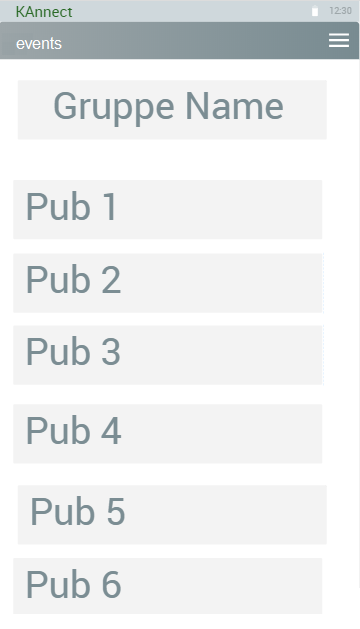
\includegraphics[height=8cm]{Group}
		\caption{Gruppe}
		\label{Gruppe}
	\end{figure}
	
	
	
	\begin{figure}[H]
		\centering
		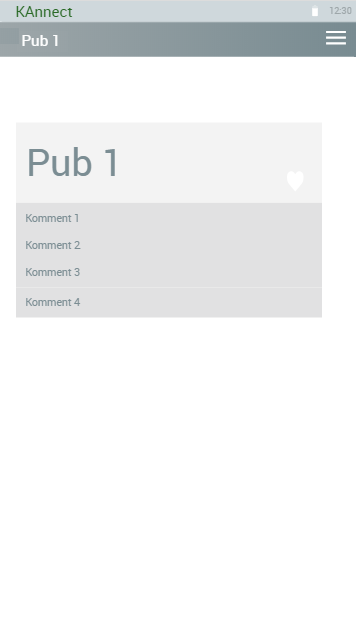
\includegraphics[height=8cm]{PubComments}
		\caption{Beitrag mit Kommentaren}
		\label{BeitragMitKommentaren}
	\end{figure}
	
	\begin{figure}[H]
		\centering
		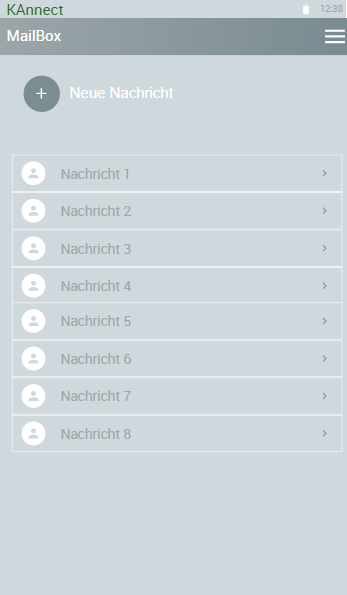
\includegraphics[height=8cm]{Briefkasten}
		\caption{Briefkasten}
		\label{Briefkasten}
	\end{figure}
	
	\begin{figure}[H]
		\centering
		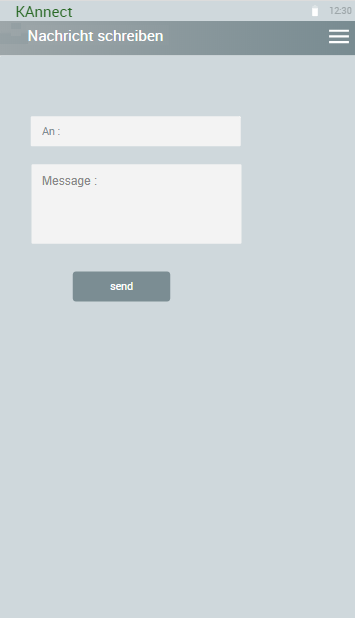
\includegraphics[height=8cm]{Message}
		\caption{Nachicht verfassen}
		\label{Nachricht}
	\end{figure}
	
	
	\newpage
	
	
	\section{Durchführbarkeitsanalyse}
	
	\subsection{Technische Durchführbarkeit}
	\subsubsection{Software}
	\begin{enumerate}[label={\alph*)}]
		\item Entwicklungstools: Programmiersprache (Kotlin), Datenbanksystem, Versionskontrolle (Git), Dokumenterstellung (LaTeX) , Photoshop ( für LOGO)
		
		\item Betriebssysteme: Windows/Linux/MacOS
		\item Web Seiten: 
		\begin{itemize} 
			\item https://www.fluidui.com/ für die Erstellung der Skizzen der grafischen Benutzeroberfläche 
			\item https://scrummate.com/ zum Verteilen der Aufgaben
			
		\end{itemize}
	\end{enumerate}
	
	\subsubsection{Hardware}
	\begin{enumerate}[label={\alph*)}]
		\item Rechner mit Internetzugang und durchschnittlicher Rechenleistung, Handy mit Android als Betriebssystem
	\end{enumerate}
	
	\subsection{Personelle Durchführbarkeit}
	\begin{enumerate}[label={\alph*)}]
		\item Projektteam : Die Projektgruppe umfasst sechs Informatikstudenten(4.Semester) und einen Betreuer(Erik Burger) als Ansprechpartner.  Jedes Projektmitglied ist  zu gleichen Teilen an der Umsetzung beteiligt . Der Zeitraum der Projektarbeit beträgt dabei ein Semester für fünf Phasen(Wasserfallmodell). Für jede Phase gibt es einen  Verantwortlichen. Jeder  Student muss insgesamt etwa  270 Stunden arbeiten.
		\item Fachliche Kompetenzen : 
		\begin{itemize}
			\item Kenntnisse aus den letzten Semestern
			\item Kenntnisse aus der Schulung (Android)
			\item Selbst angearbeitete Kenntnisse
		\end{itemize}
	\end{enumerate}
	
	\subsection{Alternative Lösungsvorschläge}
	\subsection{Risiken} 
	Auch bei einem gut geplanten und wohl strukturierten Projekt gibt es gewisse Risiken. Diese sind Ausnahmefälle. Es gibt zwei \gls{Kategorie}n :
	\begin{enumerate}[label={\alph*)}]
		\item Technische Risiken : Datenverluste durch technische Ausfälle
		\item Zeitliche Risiken : Der zeitliche Rahmen der einzelnen Entwicklungsphasen falsch eingeschätzt
		\item Personelle Risiken : Ausfallen eines Mitglieds
	\end{enumerate}
	\newpage
	
	
	\printnoidxglossaries
	
\end{document}